\documentclass[11pt,a4paper,polish,thesis]{dcsbook}

\usepackage[utf8]{inputenc}
\usepackage{babel}
\usepackage{graphicx} \graphicspath{ {images/} }
\usepackage[hidelinks]{hyperref}
\usepackage{placeins}
\setcounter{secnumdepth}{4}
\setcounter{tocdepth}{3}

\newcommand*{\captionsource}[2]{%
	\caption[{#1}]{%
		#1%
		\\\hspace{\linewidth}%
		\textbf{Źródło: } #2%
	}%
}

\begin{document}
	
	\author{Tymoteusz Bleja \and Paweł Husak \and Patryk Imosa \and Magalena Łątkowska}
	\title{Internetowa gra edukacyjna ucząca podstaw pracy~z~programem~git}
	\subtitle{Praca inżynierska}
	\supervisor{dr~hab.~inż.~Marek Andrzej Wojciechowski}
	\date{Poznań, 2017}
	\maketitle
	\frontmatter
	\tableofcontents{}
	\mainmatter
	
	\chapter{Wstęp}
	
	\section{Zasady odnośnie pisania pracy}
	
	\begin{itemize}	
		\item Piszemy w formie bezosobowej. Można też niby w 1.os liczby mnogiej czyli "Zrobiliśmy...", ale niektórzy akceptują tylko bezosobową, czyli "Zrobiono...".
		
		\item słów niepolskich - ,,Nie można więc bezpośrednio
		w tekście używać słów angielskich. Jeżeli już — powinny być wyróżnione kursywą'' - niektórzy podobno bardzo hejcą za angielskie słowa niestety.
			
		\item Jak chodzi o bibliografię, to w wolnej chwili dołączcie linki do stron z jakich korzystaliście, ja to potem ogarnę i zapiszę w takiej formie jak trzeba. Ale spokojnie, bo robienie bibliografii raczej zostawię na koniec.
		
		\item Ogólnie nie przejmujcie się strukturą, formatowaniem czy innymi formalnymi bzdetami, ja potem będę to ogarniać żeby było wg zasad więc nie traćcie czasu na ogarnianie takich rzeczy.
	\end{itemize}
	
	Między innymi: 
	skąd wgl pomysł - bo Git jest super i konieczny a ciężko się go samemu nauczyć, nauka z wielu źródeł jest chujowa, większość ma tylko blade pojęcie a potem idzie do pracy i dupa - co z tego że nauczyli się na studiach programować jak nie potrafią korzystać z Gita i współpracować z zespołem
		
	\section*{Cel i zakres pracy}
	
	cel - nauka fajna łatwa i przyjemna, oraz praktyczna, obycie z typowymi scenariuszami jakie mogą być potrzebne w pracy
	
	Coś o tym dlaczego akurat przeglądarkowa gra, czemu z grafiką 3D itp.
	
	Cytat z karty pracy : Zapoznanie się z systemem Git. Opracowanie koncepcji interaktywnego samouczka do nauki podstaw korzystania z systemu Git.  Opracowanie architektury systemu. Implementacja i testowanie systemu. Przygotowanie dokumentacji technicznej i użytkowej.
	
	\chapter{Podstawy teoretyczne}

	Systemy kontroli wersji służą do przechowywania historii plików, czyli jak sama nazwa wskazuje do kontrolowania ich różnych wersji. Dzięki temu można sprawdzić, jak zmodyfikowany został plik, a w razie potrzeby przywrócić jego poprzedni stan. Jest to szczególnie przydatne w sytuacji, w której zajdzie konieczność wycofania wprowadzonych zmian, na przykład z powodu zmiany koncepcji lub błędów.

	Systemy kontroli wersji pełnią często kluczową rolę w przypadku współpracy grupy osób nad jednym projektem. Pomagają łączyć zmiany wprowadzone przez różne osoby na tych samych plikach i służą jako narzędzie do komunikacji i synchronizacji zmian. Najczęściej są wykorzystywane przy wytwarzaniu oprogramowania, ale mogą być używane także do kontroli jakichkolwiek plików. Ich zastosowanie zastępuje popularną ze względu na swoją prostotę metodę robienia kopii zapasowych na dysku poprzez zwykłe przekopiowywanie plików.

	Wyróżnia się trzy podstawowe rodzaje systemów wersji.
	\begin{itemize}
		\item Lokalne --- umożliwiające pracę na jednym komputerze, nie pozwalające na synchronizację ze zdalnym repozytorium. Wykorzystywane są rzadko, głównie w~przypadku samodzielnej pracy nad indywidualnym projektem.
		\item Scentralizowane --- oparte na architekturze klient-serwer, w~której repozytorium przechowywane jest na jednym zdalnym serwerze, z~którym synchronizują się wszyscy użytkownicy.
		\item Rozproszone --- wykorzystujące model P2P, w~którym wszystkie komputery są sobie równoważne (nie ma jednego określonego serwera), a~kopie repozytorium znajdują się na każdej z~jednostek.
	\end{itemize}

	Porządek, w~jakim zostały one wymienione, jest nieprzypadkowy, odzwierciedla bowiem w~jakiej kolejności powstawały. Przed rozwinięciem się systemów rozproszonych przeważały systemy scentralizowane. Obecnie do wytwarzania oprogramowania przez zespoły programistów najczęściej wykorzystywane są rozproszone systemy kontroli wersji, zapewniające największe bezpieczeństwo danych. W~przypadku awarii serwera w~scentralizowanym systemie, utracone zostaje całe repozytorium. Może zostać odzyskane jedynie z~kopii zapasowych, pod warunkiem, że zostały one wcześniej wykonane. Korzystając z~rozproszonej kontroli wersji odzyskanie repozytorium po awarii jednej jednostki nie stanowi poważnego problemu, ponieważ na każdym komputerze znajduje się jego kopia.
	
	\begin{figure}
		\centering
		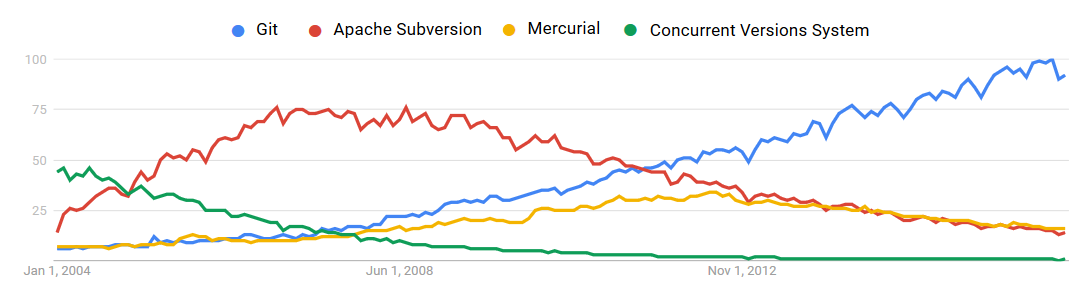
\includegraphics[width=12cm]{vcs_interest}
		\captionsource{Zainteresowanie systemami kontroli wersji w wyszukiwarce Google, dane od stycznia 2004 do stycznia 2017}{\url{https://www.google.com/trends/explore?date=2004-01-01\%202017-01-01\&q=\%2Fm\%2F05vqwg,\%2Fm\%2F012ct9,\%2Fm\%2F08441\_,\%2Fm\%2F09d6g\&hl=en-US}}
		\label{fig:vcs_interest}
	\end{figure}

	Na rysunku~\ref{fig:vcs_interest} przedstawiony jest wykres ilustrujący relatywną popularność czterech znanych systemów kontroli wersji w~wyszukiwarce Google, na przestrzeni ostatnich 13~lat. Uwzględnione zostały dwa scentralizowane (CVS i Subversion) oraz dwa rozproszone systemy kontroli wersji (Git i~Mercurial). Wyraźnie widać, że popularność tych pierwszych znacząco spadła względem rozproszonego modelu, który wciąż zyskuje na popularności. Przewaga systemu Git nad pozostałymi nie ulega wątpliwości, jest on aktualnie ponad czterokrotnie częściej wyszukiwany w~Google niż Mercurial czy Subversion, co przekłada się na stale rosnącą liczbę użytkowników.

	\section{System kontroli wersji Git}

	System kontroli wersji Git stworzony został w 2005 roku, przez zespół programistów pracujących wspólnie nad jądrem Linuksa, w~tym przez Linusa Torvaldsa, twórcę wspomnianego systemu operacyjnego. Wykorzystywali oni wcześniej inny darmowy rozproszony system kontroli wersji, który przestał być ogólnodostępny. W związku z tym postanowili napisać własny, doskonalszy od poprzedniego. Z~założenia miał to być szybki, rozproszony system, wspierający współbieżną pracę nad różnymi aspektami i~dobrze radzący sobie z~ogromnymi projektami, takimi jak jądro Linuksa.

	\subsection{Cechy charakterystyczne}
	Stworzony przez nich system kontroli wersji Git różni się znacząco od wcześniejszych systemów, szczególnie tych scentralizowanych. W odmienny sposób przechowuje nowe wersje plików. W przeciwieństwie do poprzedników zapamiętuje cały stan repozytorium, a nie jedynie różnicę pomiędzy plikami. Dla zwiększenia efektywności, jeśli plik nie został zmodyfikowany, to nie jest kopiowany tylko przechowywana jest referencja do jego aktualnej wersji.

	Kolejną istotną różnicą jest możliwość pracy lokalnej, bez ciągłej potrzeby łączenia się z~serwerem, nawet przy pracy nad projektem zespołowym. System Git pozwala wprowadzać zmiany i~zatwierdzać je bez dostępu do sieci. Komunikacja z innymi jednostkami w~celu synchronizacji danych może odbyć się w~dowolnym momencie. Wcześniejsze scentralizowane systemy, takie jak Subversion, nie pozwalały na taki model pracy, gdyż większość operacji wymagała połączenia z~serwerem, co wpływało także na dłuższy czas.

	Git przypisuje do zapisanych stanów projektu czterdziestoznakowe skróty SHA-1. Dzięki tym sumom kontrolnym zauważy każdą, nawet najmniejszą zmianę wprowadzoną na kontrolowanym pliku, niezależnie od sposobu przeprowadzenia modyfikacji.

	Jako najważniejszą zaletę systemu Git powszechnie uznaje się efektywny system rozgałęziania i~łączenia gałęzi. W~przeciwieństwie do starszych systemów kontroli wersji, Git umożliwia natychmiastowe utworzenie nowej gałęzi, oraz bardzo szybkie przełączanie się pomiędzy gałęziami. Ta cecha sprawia, że równoległa praca jest o~wiele mniej problematyczna. Znacząco ułatwia to rozwój oprogramowania jednocześnie w~kilku różnych i~niezależnych kierunkach. Tak optymalne operacje na gałęziach są możliwe dzięki potraktowaniu gałęzi jako wskaźnika na rewizję, o~czym więcej w~sekcji %\ref{Gałęzie}.

	\subsection{Repozytorium}

	Aby w pełni zrozumieć, czym jest Git, należy zacząć od wytłumaczenia kilku pojęć. Przez zwykłe repozytorium systemu Git określa się folder, przechowujący całą dotychczasową historię projektu i wszystkie zapisane wersje śledzonych plików, oraz przestrzeń roboczą (ang. \textit{working directory}), w której znajdują się bieżące pliki. Git wyróżnia także repozytoria surowe (ang. \textit{bare}), służące przede wszystkim do synchronizacji i wymiany zmian. Nie posiadają one obszaru roboczego, ponieważ nie są przeznaczone do tego, aby w nich pracować.

	Repozytorium systemu Git można samodzielnie utworzyć w dowolnym folderze na dysku, lub pobrać poprzez sklonowanie istniejącego. Pierwsza metoda może dotyczyć zarówno pustego katalogu jak i~takiego, który już zawiera projekt. Podczas inicjalizacji repozytorium zostanie utworzony osobny podkatalog .git, obejmujący wszystkie pliki potrzebne systemowi Git do działania. Pozostała zawartość folderu, w którym utworzono repozytorium, pozostanie niezmieniona. Drugi sposób polega na sklonowaniu istniejącego repozytorium do wybranego katalogu na dysku. Pobrany zostanie folder .git, wraz z całą zawartością, oraz obszar roboczy ze wszystkimi plikami projektu.

	\subsection{Tworzenie rewizji}

	Jak wspomniano wcześniej, w folderze każdego projektu kontrolowanego przez Git znajduje się podkatalog .git, zawierający całą dostępną historię i wszystkie dane dotyczące repozytorium, między innymi takie jak utworzone gałęzie. Mieści się w nim plik index. Za każdym razem, kiedy uznamy, że aktualny stan naszego projektu wart jest zapisania, trzeba samodzielnie zatwierdzić wprowadzone zmiany. Odbywa się to dwuetapowo.

	Najpierw należy określić, które pliki chce się zapisać w repozytorium, poprzez zaindeksowanie ich, czyli dodanie do indeksu (ang. \textit{index}, \textit{staging area}). Następnie zatwierdza się zmiany, w~rezultacie czego powstaje nowa rewizja (ang. \textit{commit}), zawierająca zapisany obraz całego projektu, nazywany czasem migawką (ang. \textit{snapshot}). Wszystkie rewizje przechowywane są w repozytorium i oznaczone są jednoznacznie je identyfikującą sumą kontrolną wyliczoną przez funkcję skrótu SHA-1, generującą 40-znakowy ciąg na podstawie zawartości rewizji. Poza zapisanym stanem plików zapamiętana jest także dokładna godzina zatwierdzenia zmian i autor.

	Pliki znajdujące się w projekcie kontrolowanym przez system Git można podzielić na następujące kategorie:
	\begin{itemize}
		\item aktualne - w obszarze roboczym znajduje się identyczna wersja pliku jak w ostatnio wykonanej rewizji,
		\item zmodyfikowane - od czasu zatwierdzenia zmian w pliku zostały wprowadzone pewne modyfikacje, nie dodane do indeksu (a więc gdyby w tym momencie utworzona została rewizja, to nie zawierałaby tych zmian),
		\item zaindeksowane - od czasu zatwierdzenia zmian plik został zmieniony, ale następnie dodano go do indeksu (czyli zarówno w obszarze roboczym, jak i~w~indeksie, znajduje się ta sama wersja --- będzie ona zapisana przy kolejnej rewizji).
		\item nieśledzone - pliki występujące w obszarze roboczym, ale nie znajdujące się ani w~repozytorium, ani w~indeksie --- w~tym stanie jest początkowo każdy nowo dodany do obszaru roboczego plik,
		\item ignorowane - pliki nieśledzone, wyszczególnione w~specjalnym pliku .gitignore, informującym system Git których plików ma nie uwzględniać i~nigdy nie indeksować.
	\end{itemize}

	\subsection{Gałęzie} \label{Gałęzie}
	co to gałąź, co to HEAD, stan detached HEAD

	\subsubsection{Łączenie gałęzi}
	merge i rebase

	\subsection{Repozytoria zdalne}
	co to, co to fetch, pull, push

	\subsubsection{o trackingu}


	\textit{W opisie Gita o tym czym jest repozytorium, przestrzeń robocza, indeks, indeksowanie zmian, zatwierdzanie zmian, rewizja, gałąź, HEAD, łączenie gałęzi, cofanie zmian, rebase, repozytorium zdalne, push, pull, gałąź zdalna, śledzenie gałęzi zdalnej. W nawiasach do wszystkie angielskie pojęcia.}
	
	\textit{Jakaś subsekcja o tym dlaczego programiści powinny go znać i potrafić używać jako narzędzia w pracy, do czego im się przyda i że Git często nie jest możliwością, lecz koniecznością.}
	
	\section{Gitflow}
	
	Praca z~wykorzystaniem systemu Git może przebiegać w~zgodzie ze ściśle określonym cyklem. Ustalenie reguł, których będą przestrzegać wszyscy programiści pracujący nad danym projektem, może znacząco ułatwić synchronizację pracy i~pomóc w~sprawnym zarządzaniu i~wydawaniu nowych wersji oprogramowania. Jedną z~bardziej popularnych metodyk jest Gitflow, opracowana przez Vincenta Driessena. Określa ona cykl pracy, oparty na korzystaniu z~różnych gałęzi, z~których każda ma dokładnie zdefiniowaną rolę.
	
	\subsection{Podstawowe założenia}
	
	Zamiast korzystać jedynie z domyślnej gałęzi \textit{master}, Gitflow wykorzystuje dwie główne gałęzie do rejestrowania historii projektu. Jedną z nich jest gałąź produkcyjna \textit{master}, na której przechowywane są tylko oficjalne wydania (ang. \textit{release}). Druga służy jako gałąź deweloperska i jest nazywana \textit{develop}. Przeznaczona jest do integracji bieżących prac programistycznych i nowych funkcji.
	
	Obie wspomniane gałęzie w idealnym przypadku powinny składać się jedynie z rewizji powstałych poprzez scalenie gałęzi (ang. \textit{merge commits}). Nie powinno się pracować i zatwierdzać zmian bezpośrednio na nich. Wszystkie modyfikacje kodu należy przeprowadzać na osobnych, dedykowanych gałęziach, tworzonych tymczasowo, w dokładnie określonym celu. Koncepcja Gitflow wyróżnia trzy rodzaje takich gałęzi:
	\begin{itemize}
		\item wprowadzające nowe funkcje (ang. \textit{feature branch}),
		\item przygotowujące do opublikowania nowego wydania (ang. \textit{release branch}),
		\item zawierające niezbędne i szybkie poprawki (ang. \textit{hotfix branch}).
	\end{itemize}
	Z racji braku polskich odpowiedników nazw wymienionych powyżej gałęzi, w przypadku odniesienia do nich, w dalszej części pracy wykorzystywane będzie oryginalne nazewnictwo angielskie.
	
	Z technicznego punktu widzenia typy gałęzi wykorzystywanych w Gitflow niczym się nie różnią, są to zwykłe gałęzie systemu Git. Są one szczególne jedynie pod względem konkretnych celów w jakich są używane i pewnych ograniczeń dotyczących procesu tworzenia ich i łączenia. Każdy rodzaj może powstać jedynie przez rozgałęzienie z określonej gałęzi (produkcyjnej lub deweloperskiej), a na koniec musi zostać połączony ze ściśle ustaloną gałęzią lub gałęziami.
	
	\subsection{Rozszerzanie funkcjonalności}
	
	Jednym z podstawowych założeń Gitflow jest implementowanie każdej nowej funkcji oprogramowania na osobnej, dedykowanej gałęzi typu \textit{feature branch}, której nazwa powinna zaczynać się od ,,feature/''. Taka gałąź może powstać jedynie poprzez rozgałęzienie z głównej gałęzi \textit{develop}. Z założenia ma składać się wyłącznie z rewizji zawierających zmiany dotyczące danej nowej funkcji i istnieć tak długo, jak długo trwać będzie proces implementacji.
	
	Kiedy cel zostanie zrealizowany, gałąź typu \textit{feature branch} powinna być połączona z gałęzią \textit{develop}. Istotne jest aby operacja scalania nie została wykonana poprzez przewinięcie do przodu (ang. \textit{fast forward}), czyli zwykłe przesunięcie wskaźnika HEAD. Chodzi o to by główna gałąź deweloperska nie zawierała wszystkich rewizji pochodzących z gałęzi dołączanej, a jedynie jedną powstałą jako łącznik dwóch gałęzi (ang. \textit{merge commit}). W przeciwnym wypadku określenie, które rewizje dotyczą wprowadzenia konkretnej funkcji, wymagałoby dokładnego przejrzenia zawieranych przez nie zmian. A w rezultacie znacznie trudniej byłoby usunąć pojedynczą funkcję z głównej gałęzi. 
	
	Po włączeniu zmian z gałęzi przeznaczonej do implementacji nowej funkcji do głównej gałęzi \textit{develop}, 
	należy usunąć tymczasową gałąź.
	
	\subsection{Przygotowywanie nowego wydania}
	
	Kiedy stan kodu aplikacji jest stabilny i działa zgodnie z oczekiwaniami, a wszystkie funkcje które powinny się znaleźć w nowym wydaniu oprogramowania są już zaimplementowane i włączone do głównej gałęzi deweloperskiej, należy rozpocząć proces publikacji nowej wersji. Zgodnie z koncepcją Gitflow, wszystkie niezbędne ostatnie poprawki i drobne zmiany dotyczące przygotowania nowego wydania, powinny zostać przeprowadzone na osobnej, specjalnie utworzonej w tym celu gałęzi, nazywanej \textit{release branch}.
	
	Tworzenie takiej gałęzi odbywa się poprzez rozgałęzienie z gałęzi \textit{develop}. W tym momencie ustala się też numer wydania, czyli numer wersji publikowanego oprogramowania. Nazwa gałęzi powinna być formatu ,,release/numer-wydania''.
	Od tego momentu wszystkie zmiany zachodzące na głównej gałęzi \textit{develop} będą dotyczyć następnej publikacji, nie zostaną uwzględnione w aktualnym wydaniu. Dzięki utworzeniu gałęzi typu \textit{release}, prace mogą iść dwutorowo,  poprzez przygotowywanie publikacji nowej wersji, oraz równolegle rozwijanie i rozszerzanie funkcjonalności oprogramowania. Jako przygotowanie do wydania rozumie się poprawę drobnych błędów takich jak literówki i inne niewielkie niedociągnięcia.
	
	W momencie w którym oprogramowanie będzie już przygotowane do opublikowania, należy scalić gąłąź \textit{release} z główną gałęzią produkcyjną \textit{master}. Analogicznie jak w przypadku scalania gałęzi typu \textit{feature branch}, należy  zwrócić uwagę, aby operacja połączenia nie polegała na przewinięciu do przodu. Konieczne jest aby w wyniku jej wykonania utworzona została nowa rewizja. Należy jej nadać etykietę (ang. \textit{tag}) z numerem wydania, aby ułatwić wyszukiwanie konkretnych wersji oprogramowania na gałęzi produkcyjnej. Następnie należy również scalić gałąź dotyczącą najnowszego opublikowanego właśnie wydania z gałęzią \textit{develop}. Gałęzie typu \textit{relese} są tymczasowe, więc po włączeniu jej do obu głównych gałęzi należy ją usunąć.
	
	\subsection{Naprawa błędów wymagających szybkiego rozwiązania}
	
	Kolejnym typem gałęzi wykorzystywanych w koncepcji Gitflow są gałęzie nazywane \textit{hotfix branches}, przeznaczone do naprawy niecierpiących zwłoki błędów, odkrytych w opublikowanym oprogramowaniu, najczęściej zgłoszonych przez użytkowników końcowych. Dotyczy to takich wad i problemów, które są zbyt poważne, aby mogły zostać naprawione dopiero w następnym wydaniu. W przypadku mniej istotnych niedociągnięć wystarczy poprawić dane aspekty w normalnym trybie pracy i włączyć je do gałęzi \textit{develop}, żeby zostały uwzględnione przy kolejnej publikacji przez gałąź typu \textit{release}. 
	
	Gałąź typu \textit{hotfix} jest jedynym rodzajem gałęzi, który powstaje poprzez rozgałęzienie z głównej gałęzi produkcyjnej \textit{master}. Jej nazwa powinna zaczynać się od wyrażenia ,,hotfix/''. Taka gałąź zawiera tylko zmiany dotyczące naprawy wykrytego błędu, które powinny być wykonane w możliwie najkrótszym czasie. Kiedy problem zostanie rozwiązany, przeznaczoną mu gałąź należy połączyć z powrotem z gałęzią \textit{master}. W tym przypadku również należy dokonać łączenia nie poprzez przewijanie do przodu. W rezultacie na głównej gałęzi produkcyjnej powstaje nowa rewizja, której należy nadać etykietę z nowym numerem wersji. Skutkiem jest publikacja nowego wydania oprogramowania, która, w przeciwieństwie do procesu z wykorzystaniem gałęzi typu \textit{release} nie była planowana. 
	
	Kolejnym krokiem jest scalenie gałezi \textit{hotfix} z główną gałęzią \textit{develop}. Jeżeli istnieje w danym momencie gałąź typu \textit{release}, to do niej również należy włączyć zmiany dotyczące naprawy błędu. Na koniec należy usunąć tymczasową gałąź.
	
	\chapter{Projekt}
	
	\section{Założenia}
		
	Głównym celem samouczka GITar-Hero jest zapoznanie użytkownika z~podstawowymi poleceniami systemu kontroli wersji Git, w~sposób przyjemny i~zrozumiały. Gra, przez połączenie nauki i rozrywki, ma za zadanie zachęcić i ułatwić proces uczenia się. Kolorowa i ruchoma grafika 3D uatrakcyjnia tę naukę, a możliwość zdobywania punktów i naturalna chęć osiągnięcia jak najlepszego wyniku dodatkowo mobilizuje użytkownika. 
	
	Z założenia, ważniejsze od dogłębnego zrozumienia strony teoretycznej systemu Git, było nauczenie właściwego korzystania z poleceń. Gra ma służyć jako samouczek, uczący praktycznego wykorzystania systemu wersji i~pokazujący typowy scenariusz, jaki najczęściej występuje podczas wytwarzania oprogramowania. Po zagraniu w grę użytkownik powinien już swobodnie wykonywać komendy systemu Git, zarówno pracując indywidualnie, jak i potrafić właściwie współpracować z zespołem. 
	
	Celem było pokazanie, że wbrew panującej powszechnie opinii, korzystanie z systemu kontroli wersji Git nie musi przysparzać problemów ani trudności. Ponadto gra ma przyzwyczaić użytkownika do korzystania z wiersza poleceń. Jeżeli ma się opanowane komendy, jakie należy wprowadzać w konsoli, z reguły będzie się potrafiło skorzystać z dowolnego programu z graficznym interfejsem do obsługi systemu Git. W drugą stronę taka zależność nie występuje. W związku z tym, tylko umiejętność korzystania z systemu Git w wierszu poleceń pozwala swobodnie korzystać z tego systemu kontroli wersji, niezależnie od środowiska i zainstalowanych programów.
	 
	\section{Przebieg gry}
	
	Gra zaczyna się od krótkiego wprowadzenia, informującego użytkownika, na czym będzie polegała rozgrywka i do czego służą poszczególne elementy interfejsu. Po zapoznaniu się z krótką instrukcją rozpoczyna się gra. U góry, po prawej stronie, wyświetla się aktualne zadanie i pierwszy krok, który należy wykonać. Z założenia użytkownik nie zna poleceń systemu Git, dlatego automatycznie otwiera się pomoc z zakładką informującą czym jest repozytorium sytemu kontroli wersji i jak je zainicjować. Pomoc zawiera wszystko, co gracz musi wiedzieć, aby poprawnie wykonać dany krok. Po wprowadzeniu przez niego właściwego polecenia i zatwierdzeniu go poprzez przycisk Enter, aktualny krok zostaje zaliczony i następuje przejście do kolejnego. Dodatkowo w katalogu projektu, po lewej stronie, pojawiają się aktualne pliki, jakie znajdują się na tym etapie w folderze z repozytorium. Poza tym akcje wykonywane na repozytorium są odwzorowywane przez grafikę 3D, która reaguje odpowiednio na wpisane komendy. Obrazuje to, jak wywołane polecenie działa na stan repozytorium i pozwala użytkownikowi lepiej zrozumieć skutki wykonywanych komend. 
	
	Po poprawnym wykonaniu przez użytkownika wszystkich kroków zadania, otrzymuje on punkty. Ich liczba jest zależna od czasu, jaki pozostał do końca zadania. Im szybciej gracz ukończy, tym więcej punktów dostanie. Możliwe jest także nie otrzymanie żadnych punktów za wykonanie zadania, jeżeli przekroczony zostanie przydzielony do niego czas. 
	
	Kolejne zadania stopniowo wprowadzają nowe komendy. Ich poziom trudności rośnie, zawierają one coraz więcej kroków. Jeżeli użytkownik nie będzie potrafił wykonać aktualnego kroku, może w dowolnej chwili wpisać w konsoli 'help'. Otworzy się wówczas pomoc i~gracz będzie mógł poszukać potrzebnych mu informacji. 
	
	Po przejściu całego scenariusza wyświetli się podsumowanie, zawierające liczbę zdobytych przez gracza punktów oraz podstawowe statystyki, zawierające informację o liczbie popełnionych błędów i komendach, z~którymi miał najwięcej problemów. 
	
	\section{Zadania}
	
	Scenariusz rozgrywki składa się z zadań zawierających niezbędne komendy do typowego wykorzystania systemu kontroli wersji Git. Użytkownik uczy się najpierw o tym, czym jest repozytorium. Poznaje dwie podstawowe metody pozyskania takiego repozytorium --- poprzez sklonowanie istniejącego lub przez założenie go w wybranym folderze z~projektem. W~kolejnym etapie zapoznaje się z~pojęciami takimi jak przestrzeń robocza, indeks, indeksowanie plików, zatwierdzanie zmian i~rewizja. Potrafi rozróżnić co oznacza plik aktualny, zmodyfikowany, nieśledzony lub niezaindeksowany. Przed wprowadzeniem kolejnych poleceń i~terminów zadania koncentrują się na tej tematyce, aby użytkownik zdążył je dobrze opanować. 
	
	Po wykonaniu kilku zadań dotyczących wspomnianych wyżej zagadnień, użytkownik uczy się o~gałęziach, poznaje sposoby tworzenia ich i~przełączania się między nimi. Wprowadzane są też pojęcia takie jak gałąź tematyczna, poświęcona konkretnej dodatkowej funkcji aplikacji (ang. \textit{feature branch}). Przy okazji nadal utrwalane są komendy przedstawione w pierwszych zadaniach, dotyczące indeksowania plików i~zatwierdzania zmian. 

	Kolejnym etapem jest nauka scalania, lub inaczej łączenia gałęzi. Rozróżnione są przy tym odmienne sposoby na wykonanie tej operacji. Następnie pojawia się podstawowy sposób wycofywania zmian i~usuwania wykonanych wcześniej rewizji. 
	
	Kiedy użytkownik opanuje już komendy i~sposób pracy w lokalnym repozytorium, wprowadzane jest pojęcie zdalnego repozytorium oraz sposoby komunikacji i~synchronizacji z~nim. W~zadaniach pojawiają się komendy dotyczące ściągania i~przesyłania zmian. Poruszany jest także temat zdalnych gałęzi i~sposoby skonfigurowania lokalnej gałęzi śledzącej zdalną.
	
	Ponadto podczas nauki poleceń systemu Git użytkownik zapoznaje się też z~dobrymi praktykami i~metodyką Gitflow, co uczy go właściwych nawyków i~odpowiedniego porządkowania pracy nad projektem. Zaznajamia się z~koncepcją tworzenia osobnych gałęzi przeznaczonych do implementacji nowych funkcji lub naprawy błędów.
	
	Zadania są podzielone na kroki, dzięki czemu użytkownik uczy się charakterystycznych sekwencji poleceń, często występujących razem. Ma to również na celu zautomatyzowanie zachowania użytkownika w prawdziwych przypadkach, z którymi może się spotkać w domu lub pracy. W systemie Git czasem możliwe jest użycie kilku różnych poleceń, aby osiągnąć ten sam rezultat. Zadania i kroki dopuszczają wszystkie właściwe komendy.
	
	\subsection{Pomoc}
	
	Wszystkie materiały dydaktyczne znajdują się w pomocy. Jest ona podzielona na zakładki, z~których każda dotyczy jednej komendy lub pojęcia. Treść zawarta w niej wystarcza, aby osoba nie znająca poleceń systemu Git była w stanie poprawnie wykonać zadania ze scenariusza rozgrywki. W przypadku niektórych pojęć jest jednak bardziej obszerna i wykracza poza wymaganą do przejścia gry wiedzę. Zawiera informacje, które uznano za szczególnie istotne i przydatne do właściwego zrozumienia systemu Git.
	
	Za każdym razem, gdy podczas rozgrywki w jednym z kroków zadania pojawia się nowe polecenie, pomoc otwiera się automatycznie na odpowiedniej zakładce. Użytkownik może poświęcić dowolnie dużo czasu na zaznajomienie się z~jej treścią, a~ponadto w każdej chwili ma możliwość ponownego przeczytania informacji dotyczących wcześniejszych poleceń.  
	
	\subsection{Punkty za rozwiązanie}

	%Tak w ogóle to chyba najpiej wywalić subsekcje o punktach, a ten akapit poniższy dać gdzie indziej
	W projekcie wprowadzono elementy gamifikacji, takie jak punkty za rozwiązanie zadań. Mają one za zadanie zwiększyć zaangażowanie użytkownika. Z każdym rozegraniem, gracz będzie starać się poprawić swój dotychczasowy wynik. W ten sposób co raz szybciej i pewniej będzie korzystał z poleceń systemu Git. Ponadto punkty wprowadzają element rywalizacji pomiędzy użytkownikami, którzy będą dążyć do tego aby zająć jak najwyższe miejsce w rankingu. 
	
	Punkty obliczane są na podstawie czasu, w jakim użytkownik rozwiązał zadanie. 
	
	
	%Ten akapit chyba do wywalenia, a na pewno do zmiany -najpierw trzeba wgl ustalic jak to będzie z tymi punktami
	\textit{	Został dla nich stworzony komponent, który reaguje na zakończenie zadania. Przy wybieraniu zadania jako kolejne ustawiana jest wartość nagrody za poprawne wykonanie całego zadania. Wartość ta obliczana jest na podstawie minimalnego czasu przeznaczonego na dane zadanie pomnożonego przez ilość wykonanych zadań oraz liczbę 10. Co daje nam możliwość premiowania zadań, które są są wykonywane głębiej naszego drzewa zadań oraz mają być wykonane szybciej niż inne zdania. Gdy zadanie zostaje wykonane pobierany jest czas wykonania zadania. Jeżeli zadanie zostaje wykonane po przekroczeniu określonego na zadanie czasu użytkownik nie otrzymuje punktów. Natomiast jeżeli użytkownik zmieścił się w czasie, obliczona wcześniej nagroda zostaje pomnożona przez stosunek czasu, który został do czasu przeznaczonego na zadanie. Całość jest zaokrąglana w górę do liczby całkowitej. Obliczona wartość jest dodawana do całkowitej ilości punktów jaką dotychczas zdobył gracz. }
	
	\chapter{Implementacja}
	
	\section{Wykorzystane technologie}
	
	\subsection{Języki}
	
	\subsubsection{JavaScript}
	
	\subsubsection{GLSL}
	
	\subsection{Biblioteki}
	
	\subsubsection{Redux}
	
	Wymagania dotyczące aplikacji przeglądarkowych stały się na tyle skomplikowane, że interfejs użytkownika jest bardzo złożony i może składać się z wielu elementów. Zarządzanie stanem takich aplikacji jest trudne, ponieważ występuje wiele zależności między komponentami. Może to doprowadzić do sytuacji, w której nie jest jasne co tak naprawdę się dzieje, a znalezienie błędów czy rozszerzenie funkcjonalności staje się zadaniem bardzo czasochłonnym i karkołomnym. 
	
	Jednym z rozwiązań jest właśnie skorzystanie z biblioteki Redux dla aplikacji pisanych w języku JavaScript. Głównym jej założeniem jest przejrzysty stan aplikacji, który może zmieniać się tylko w określonych momentach i~zawsze w~przewidywalny sposób. 
	
	Stan jest zdefiniowany jako zwykły obiekt o~strukturze drzewa, zawierający wszystkie możliwe informacje, jakie są potrzebne aby jednoznacznie określić i móc odtworzyć identyczną sytuację w aplikacji. Nie może on być modyfikowany, jest tylko do odczytu. Jedynym sposobem na jego zmianę jest wyemitowanie akcji, będącej po prostu zwykłym obiektem zawierającym obowiązkowo pole typ i dowolne inne potrzebne atrybuty.	Zadaniem akcji jest przejrzysty opis tego, co się wydarzyło w aplikacji, dzięki czemu dokładnie wiadomo co spowodowało zmianę. 
	
	Kluczowym elementem Reduxa są specyficzne funkcje, nazywane w języku angielskim \textit{reducers}, które definiują jak konkretna akcja wpływa na stan. Każda funkcja \textit{reducer} musi spełniać określone wymagania. Jako parametry przyjmuje zawsze tylko i~wyłącznie obecny stan aplikacji i wyemitowaną akcję, a zwraca nowy obiekt stanu, w jakim znajduje się aplikacja na skutek wykonanej akcji. Ważne jest także aby \textit{reducer} był przewidywalny i~deterministyczny. Oznacza to, że określony stan aplikacji i~określona akcja spowodują powstanie zawsze takiego samego stanu. Dodatkowo taka funkcja nie może mieć żadnych skutków ubocznych. W dużych projektach wskazane jest napisanie kilku takich funkcji, z~których każda wpływa tylko na określoną część stanu. Ułatwia to utrzymanie zrozumiałego kodu, który można łatwo rozwijać i~modyfikować.
	
	Podsumowując, Redux opiera się na trzech fundamentalnych zasadach:	
	\begin{itemize}
		\item cały stan aplikacji jest opisany przez pojedynczy obiekt o strukturze drzewa,
		\item jedynym sposobem aby zmienić stan aplikacji jest wyemitowanie akcji,
		\item wpływ danej akcji na sposób przekształcenia stanu określają funkcje zwane \textit{reducers}.
	\end{itemize}

	Popularność biblioteki Redux zasłużenie rośnie, ze~względu na~prostotę i~korzyści, jakie daje przestrzeganie opisanych wyżej trzech podstawowych reguł. Zdecydowano się skorzystać z~tej biblioteki ponieważ jest łatwa w~użyciu i~pozwala w~wygodny sposób zarządzać stanem aplikacji. 
	
	\subsubsection{React.js}
	 
	 Jako bibliotekę do budowania interfejsu użytkownika wybrano bibliotekę React. 
	 Została ona stworzona w 2013 roku przez zespół programistów Facebook'a, aby rozwiązać problem tworzenia dużych aplikacji, w których nieustannie zmienia się to, co należy wyświetlać. Początkowo nie była ona ogólnodostępna, ale aktualnie jest udostępniona na zasadzie otwartego źródła (ang. \textit{open-source}) w serwisie github.com. React pozwala określić jak aplikacja powinna wyglądać w różnych momentach, a samo odświeżanie interfejsu dzieje się automatycznie, gdy zmienią się dane dotyczące komponentów. Dodatkowo ogromną zaletą tej biblioteki jest fakt, że potrafi ona określić co dokładnie uległo zmianie, a~w~rezultacie ponownie wyrenderowć tylko fragmenty, które rzeczywiście tego wymagają.
	 
	 React opiera się na koncepcji niezależnych komponentów, nadających się do~wielokrotnego wykorzystania, z~których można komponować skomplikowane widoki. Są to obiekty JavaScript, reprezentujące elementy HTML, czyli w~istocie fragmenty interfejsu użytkownika, mające określoną strukturę i~funkcjonalność.
	 
	 Wykorzystywany jest też wirtualny obiektowy model elementu (ang. \textit{virtual DOM}), czyli obiekt o strukturze drzewa, zbudowany z wcześniej zdefiniowanych komponentów. React obserwuje, czy nie nastąpiły żadne zmiany w~nim, a~jeżeli tak, to automatycznie modyfikuje rzeczywisty i~widoczny dla użytkownika DOM, tak aby odzwierciedlał on stan wirtualnego DOM. Istotne jest, że~odświeżeniu podlegają tylko te fragmenty, które uległy zmianie.
	 
	 Kluczową rolę pełni funkcja \textit{render}, przyjmująca dwa parametry --- wirtualny element oraz węzeł DOM, w którym umieszczony zostanie dany element. Dopiero jej wywołanie powoduje, że komponent jest widoczny w przeglądarce. Każdy z takich elementów może mieć właściwości (ang.\textit{props}) oraz przechowywać swój własny wewnętrzny stan (ang. \textit{state}). Różnica między nimi jest taka, że właściwości powinny być stałe, a stan może się zmieniać w czasie. Jego zmiana wywołuje metodę \textit{render()}, odświeżającą komponent.
	
	Zdecydowano się na wykorzystanie biblioteki React.js, ponieważ aplikacje napisane z~jej użyciem wymagają mniejszego nakładu pracy aby działać responsywnie i szybko. Dodatkowo biblioteka ta doskonale współpracuje z Reduxem, w którym stan całej aplikacji przechowywany jest w jednym obiekcie nazywanym stanem. Wystarczy odpowiednie jego fragmenty podpiąć do konkretnych komponentów, aby interfejs automatycznie reagował na jego zmiany. 
		
		
	\subsubsection{Babylon.js}

	Babylon.js jest otwartą biblioteką WebGL napisaną w TypeScript i~wykorzystywaną przede wszystkim do tworzenia gier wideo w~przeglądarkach. Pierwsza odsłona została wydana w~2013~roku. Głównymi twórcami są David Cotuhe oraz David Rousset. Jako, że Babylon.js jest silnikiem 3D, posiada wspaniałe narzędzia do tworzenia, wyświetlania i~teksturowania szkieletów w~przestrzeni. Przez to, że~kierowana jest głównie do twórców gier, posiada wiele dodatkowych funkcji takich jak generowanie krawędzi czy tworzenie obiektu na podstawie mapy wysokości. Ponadto zapewnia natywną detekcję kolizji, grawitację sceny oraz wbudowane kamery, takie jak kamera śledząca, automatycznie podążająca za obiektem. 
	
	Rozważana była jeszcze inna biblioteka 3D, a mianowicie Three.js wydana w 2009 roku, również oparta na~webGL. Po zapoznaniu i~przetestowaniu obu silników wybór padł na Babylon.js. Przyczyniły się do tego przede wszystkim prostota użycia oraz płynność, którą zapewniał w przeciwieństwie do Three.js. Przy renderowaniu tego samego, wybranego obiektu, Babylon.js spisywał się lepiej o kilka klatek. Poza tym biblioteka ta jest dobrze udokumentowana i~posiada bogatą bazę poradników, a~społeczność wykorzystująca tę bibliotekę jest bardzo liczna i~stale rośnie.
	
	\subsubsection{Pozostałe}
	
	\section{Scenariusz rozgrywki}
	
	\subsection{Struktura} \label{Struktura}
	
	Scenariusz rozgrywki to skierowany graf, którego wierzchołkami są zadania, z~których każde składa się z~kilku kroków. Zdecydowano się na taką strukturę ze względu na to, że daje ona możliwość sekwencjonowania zadań, a zarazem pozwala na element losowości. Jeżeli z wierzchołka dotyczącego jakiegoś zadania wychodzi kilka krawędzi, to kolejny węzeł, czyli kolejne zadanie, wybierane jest w sposób losowy spośród sąsiadów aktualnego wierzchołka. Dzięki takiej reprezentacji nigdy nie zdarzy się sytuacja, w której następnym zadaniem będzie zadanie nieadekwatne do aktualnego stanu repozytorium.

	\subsubsection{Konstrukcja zadania}
	Pojedyncze zadanie reprezentowane jest w postaci obiektu, który składa się z następujących pól:
	\begin{itemize}
	\item identyfikator,
	\item zbiór identyfikatorów możliwych następników,
	\item tytuł,
	\item opis,
	\item minimalny czas,
	\item domyślny (maksymalny) czas,
	\item lista kroków.	
	\end{itemize}
	
	Opis zadania służy ukazaniu użytkownikowi celu oraz problemu, jaki należy rozwiązać w danym zadaniu. Może to być na przykład rozszerzenie funkcjonalności lub naprawa błędu.
	
	%Tu też do zmiany jak ustalimy co z punktami
	\textit{Aby nagradzać użytkownika punktami za szybko wykonane zadanie, zdecydowano się na określenie czasu na wykonanie zadania. Jest on obliczany w momencie dodawania nowego zadania na podstawie ilości dotychczas wykonanych zadań, a także wartości minimalnej oraz maksymalnej czasu zdefiniowanych w danym zadaniu.}
	
	Zbiór następników zawiera identyfikatory zadań, które mogą wystąpić po aktualnym. Hierarchia zadań ułożona jest w postaci grafu skierowanego, tak więc wszystkie wierzchołki, do których istnieją krawędzie wychodzące z wierzchołka reprezentującego dane zadanie, są jego następnikami. 
	
	Kluczowym elementem zadania jest uporządkowana lista kroków, które należy wykonać, aby rozwiązać zadanie i przejść do kolejnego. Wykonanie kroku polega na wpisaniu odpowiedniej komendy systemu Git. Szczegółowy opis jego konstrukcji w kolejnej sekcji.

	
	\subsubsection{Konstrukcja kroku}
	
	Podobnie jak zadanie, krok jest obiektem składającym się z kilku pól, a mianowicie:
	\begin{itemize}
		\item typ,
		\item opis,
		\item lista dozwolonych poleceń,
		\item etykiety,
		\item dodatkowe dane, charakterystyczne dla danego typu kroku.	
	\end{itemize}

	Typ określa jakiej komendy systemu Git dany krok dotyczy. Obsługiwane typy to m.in. ''COMMIT'' czy ''MERGE''. Na podstawie typu poprawnie wykonanego kroku określana jest akcja, jaką należy wykonać po stronie grafiki 3D, by odwzorować aktualny stan repozytorium. 
	 
	W opisie znajduje się krótka informacja, co należy zrobić, aby wykonać krok i przejść do kolejnego. Krok jest uznawany za wykonany, gdy użytkownik wpisze w konsoli jedno z~poleceń z~listy dozwolonych komend i~zatwierdzi je.
	
	Do każdego kroku przypisana jest lista etykiet, określających jakiego zagadnienia dotyczy dany krok. Krok posiada zawsze co najmniej jedną etykietę, wskazującą komendę, której wymaga on do poprawnego wykonania. Gdy użytkownik poprawnie zrealizuje dany krok, to zwiększany jest wskaźnik powodzenia dla wszystkich przypisanych do niego etykiet. Poza wspomnianym wskaźnikiem przechowywana jest także ilość poprawnych wywołań komendy. Informacje te umożliwiają określenie stopnia, w jakim użytkownik opanował dane zagadnienie i nad czym powinien jeszcze popracować. Brane jest to pod uwagę przy losowaniu kolejnych zadań. Dla możliwych następników wyliczana jest waga na podstawie etykiet, jakie mają w swoich krokach. 
	
	\textit{Obliczenie wagi dla zadania polega na zsumowaniu kwadratów ilorazu wartości 1 oraz wyznaczonego wskaźnika dla kolejnych etykiet w krokach zadania, będącego ilorazem poprawnie wykonanych kroków z całkowitą liczbą prób dla tej etykiety. Dzięki takiemu zabiegowi zwiększane jest prawdopodobieństwo wylosowania kolejnego zadania poruszającego zagadnienia, z~którymi użytkownik nie radził sobie zbyt dobrze.}
	
	Dodatkowe dane, w zależności od typu kroku, mogą składać się z różnych elementów. Dostarczają informację np. o nazwie wykonanej rewizji czy utworzonej gałęzi. Służą też do określenia jakie pliki powinny zostać dodane lub usunięte z repozytorium. W przypadku kroku dotyczącego polecenia \textit{git checkout} przechowują informację, czy przełączenie powinno być zrealizowane na konkretną gałąź czy rewizję.
	
	\subsubsection{Format danych}
	
	Jak opisano wcześniej, scenariusz rozgrywki to w istocie struktura drzewiasta złożona z zadań, przy czym każde z nich zawiera pewne informacje oraz uporządkowaną listę kroków. Tak złożony obiekt wymagał odpowiedniego i wygodnego formatu do przechowywania danych. Zdecydowano się na format JSON, który doskonale nadaje się do tego celu. Pliki zapisane w tym formacie można bezproblemowo odczytywać oraz modyfikować za pomocą języka JavaScript.
	
	\subsection{Graficzne narzędzie do definiowania scenariuszy}
	
	\subsubsection{Motywacja}
	
	Aplikacja GITar Hero umożliwia przetwarzanie rozbudowanych scenariuszy, których ręczne tworzenie byłoby uciążliwe i  czasochłonne, a ponadto podatne na błędy. Dodawanie lub modyfikacja zadań wymagałaby znaczących nakładów pracy.
	Z tego względu zdecydowano się na korzystanie z narzędzia z graficznym interfejsem użytkownika, za pomocą którego można by było w prosty i wygodny sposób tworzyć grafy zadań oraz zapisywać je w formacie JSON. 
	
	\subsubsection{Poszukiwanie gotowego rozwiązania}
	
	Początkowo zamierzano skorzystać z gotowego rozwiązania. Do tego zadania wytypowano aplikację \textit{directed-graph-creator} użytkownika cjrd [tu odnosnik do bibliografii i tam link] udostępnianą jako oprogramowanie o~otwartym źródle (ang. \textit{open source}) \footnote{Oprogramowanie udostępnione jest na licencji MIT/X, dzięki czemu istnieje nieograniczone prawo do używania, kopiowania, modyfikowania i~rozpowszechniania go. Jedynym wymogiem jest, by we wszystkich wersjach zachowano warunki licencyjne oraz informacje o autorze.}. Umożliwia ona tworzenie grafów skierowanych oraz~ich zapis do formatu JSON. Narzędzie to jest zaimplementowane w języku JavaScript i~korzysta z popularnej biblioteki~D3.js, która pozwala tworzyć dynamiczne i~interaktywne wizualizacje danych w~przeglądarkach internetowych.
	
	Jednakże aplikacja, w~formie w jakiej została udostępniona, nie wystarczała do zdefiniowania scenariusza rozgrywki. Każdy węzeł grafu mógł przechowywać tylko pojedynczy ciąg znaków. Potrzebne były zatem znaczne modyfikacje, umożliwiające zapisanie w pojedynczym węźle wszystkich niezbędnych informacji, które powinny się znaleźć w zadaniu. Zdecydowano się zatem stworzyć własne narzędzie do~tworzenia scenariusza zadań, bazujące na ogólnodostępnym \textit{direct-graph-creator}.
	
	\subsubsection{TaskCreator}
	
	Postanowiono przerobić wspomnianą wyżej aplikację. Została ona napisana tylko i wyłącznie w języku JavaScript, bez wykorzystania jakichkolwiek platform programistycznych (ang. \textit{frameworks}). Modyfikację utrudniał także fakt, że cały kod zawarty był w~jednym pliku. Postanowiono nie modyfikować struktury aplikacji i~dalszą część napisać również w czystym języku JavaScript. Dodano jedynie bibliotekę jQuery, która umożliwia łatwiejsze zarządzanie elementami drzewa DOM, czyli obiektowego modelu dokumentu. W~związku z~tym, że jest to aplikacja internetowa, potrzebny był serwer HTTP. W~tym celu użyto środowiska Node.js, wykorzystywanego do tworzenia wysoce skalowalnych aplikacji sieciowych.
		
	\begin{figure}
		\centering
		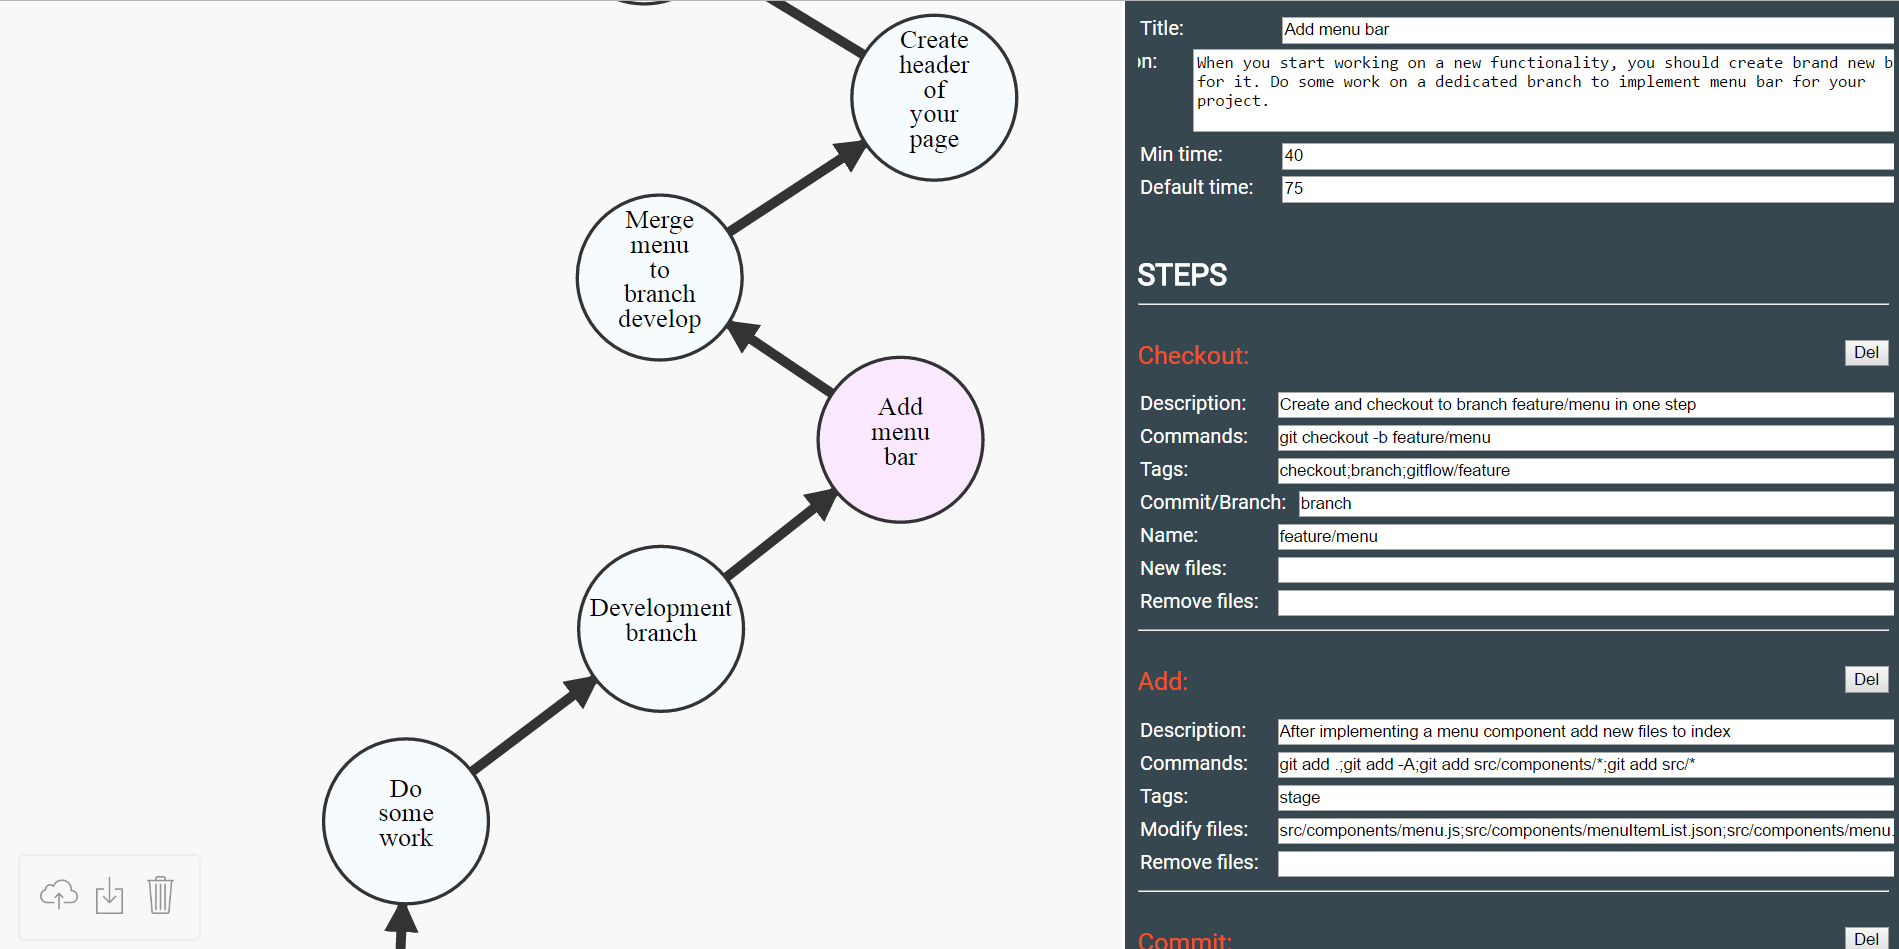
\includegraphics[width=12cm]{graphCreator01}
		\caption{Interfejs graficzny narzędzia TaskCreator}
		\label{fig:taskCreator}
	\end{figure}
	
	Największą modyfikacją było rozszerzenie interfejsu o dodatkowy panel boczny służący do wypełniania pól zadania i definiowania listy kroków. Jest on widoczny na rysunku~\ref{fig:taskCreator} po prawej stronie. Po~kliknięciu na węzeł grafu, reprezentujący pojedyncze zadanie, na bocznym panelu zostają wyświetlone wszystkie informacje dotyczącego wybranego elementu. Należą do nich między innymi tytuł, opis oraz czasy wykonania. Oczywiście wszystkie pola są edytowalne. W panelu istnieje również możliwość definiowania listy kroków, które trzeba zrealizować żeby wykonać zadanie. Aby dodać jeden z nich należy wybrać jego typ i kliknąć przycisk "Dodaj", a następnie wypełnić pola opisujące dany krok. Znajdują się tam atrybuty takie jak opis, lista komend spełniająca dany krok, etykiety opisujące wykonane czynności jak również dodatkowe parametry, charakterystyczne dla poszczególnych typów kroków. 
	
	Aby dodać nowy węzeł grafu należy przytrzymać klawisz Shift i kliknąć myszką w wybrane miejsce. Żeby edytować wierzchołek należy go wybrać poprzez kliknięcie. Z kolei przytrzymanie klawisza Shift oraz wciśniętego lewego przycisku myszki a następnie przeciągniecie kursora znad jednego węzła na drugi utworzy skierowaną krawędź między nimi. Aby usunąć wybrany wierzchołek grafu bądź jego krawędź, należy go zaznaczyć kliknięciem oraz nacisnąć klawisz Delete. 
	
	Stworzony w ten sposób graf zadań można zapisać do formatu JSON. W tym celu wystarczy kliknąć drugi przycisk w lewym dolnym rogu ekranu. Narzędzie wygeneruje strukturę grafu zrozumiałą dla aplikacji GITar Hero, określi zadanie inicjujące rozgrywkę i zapisze dane do pliku taskGraph.json. Zapisane w ten sposób grafy można wczytać ponownie do aplikacji TaskCreator naciskając pierwszy przycisk w lewym dolnym rogu ekranu i wybierając plik do wczytania.
	
	\section{Komponenty/elementy(?) aplikacji}
	
	\subsection{Lista zadań}
	
	Screen jakiś, jak działa, o implementacji
	
	\subsection{Konsola}
	
	Screen jakiś, jak działa, o implementacji
	
	\subsection{Pomoc (HelpDrawer)}
	
	Screen jakiś, jak działa, o implementacji
	
	\subsection{Drzewko repo}
	
	Screen jakiś, jak działa, o implementacji
	
	\subsection{Canvas}
	
	W projekcie skorzystano z komponentu 'canvas' z html w wersji 5. Pozwala on na wyświetlanie grafiki w przeglądarce. Służy jako kontener dla graficznego silnika 3D, pochodzącego z biblioteki babylon. 
	
	\section{Grafika 3D}
	Tu będzie sporo, do tego stopnie sporo, że nie wiem jeszcze jak to zaplanować i porozdzielać, względem czego.
	
	Czy np podsekcje takie jak:
	repo3d - gałęzie, commity, co to są i jak powstają na akcje, o ich teksturze, obramowaniu, w tym o solidExplode
	ground - co to, jak działa itp
	particle w tle
	(wg elementów aplikacji)
	
	Czy może raczej podsekcje wg 'elementów' Babylona:
	Meshe, SolidParticle, Particle, Materiały, Tekstury, Shadery
	
	

	\subsection{Repozytorium 3D}
		Aby odwzorowywać stan repozytorium na ekranie został stworzony odpowiedni kontroler. Ma on za zadanie reagować na realizowane przez użytkownika komendy i zarządzać elementami grafiki 3D. Nasłuchuje na wykonywane akcje i w zależności od ich typu dodaje, usuwa bądź modyfikuje elementy na scenie. W kontroler ten zawiera listę gałęzi będących w stanie repozytorium. % husaku i imosiaku

	\subsection{Branch}
	Obiekt 3D reprezentujący gałąź systemu git jest tworzony przy pomocy funkcji CreateTube z biblioteki Babylon.js. 
	Funkcja ta generuje siatkę wierzchołków, na podstawie podanej listy punktów określających ścieżkę, w kształcie tuby. Pozwala również na określenie średnicy oraz
	szczegółowości siatki. Parametry te zostały dobrane w taki sposób, aby wygenerować tubę, której przekrój przypomina koło przy jednoczesnym zachowaniu jak najmniejszej liczby użytych wierzchołków. Jedna gałąź może składać się z dwóch rodzajów siatki. Pierwsza z nich reprezentuje główny człon. Ścieżka użyta do jej wygenerowania zawiera tylko dwa punkty wyznaczające początek i koniec tuby. Dzięki temu można osiągnąć dowolnie długi odcinek nie zwiększając przy tym liczby wierzchołków. SPRAWDZIC I OPISAC PROBLEM Z IN FRUSTRUM. Drugi rodzaj siatki wykorzystywany jest do wygenerowania tuby będącej łącznikiem między gałęziami. Łącznik branchy zostaje stworzony w momencie tworzenia nowej gałęzi lub łączenia dwóch gałęzi w akcji merge. Do wyznaczenia ścieżki skorzystano z funkcji pomocniczej generującą krzywą Beziera. Funkcja ta przyjmuje cztery punkty na podstawie których wyznaczy tablicę punktów tworzących linie. Jako pierwszy punkt podane jest miejsce początku nowej gałęzi, dwa kolejne punkty służą do określenia kształtu lini. Jako ostatni punkt podawany jest początkowy punkt głównego członu nowej gałęzi. Dodatkowym parametrem jest ilość wygenerowanych punktów określającym szczegółowość linii. Dzięki tej funkcji otrzymano tablicę punktów, która została użyta do określenia kształtu łącznika.
	
	Na gałąź nałożono standardowy materiał. Jest to klasa z biblioteki Babylon.js reprezentująca uniwersalny shader, używany do rysowania wierzchołków. Można w niej ustawić takie parametry jak kolor rozproszonego światła,  
	Na końcu gażdej gałęzi wyświetlana jest tekst z nazwa gałęzi. Jego pozycję ustawiono na referencję do ostatniego punktu gałęzi dzięki czemu tekst zawsze podąża za wydłużającą lub skracającą się gałęzią. 
	
	
	%standardowy material 
	% tuba
	% connectory
	% tekst
	% husaku i imosiaku

	\subsection{Commit}
	Zatwierdzenie zmian w repozytorium git w grafice trójwymiarowej jest przedstawione w postaci kuli umieszczonej na gałęzi, której dotyczy. Funkcja CreateSphere pochodząca z babylon'a buduje siatkę wierzchołków w kształcie sfery o określonej średnicy oraz teselacji. Przy wartości teselacji równej szesnaście powierzchnia obiektu wygląda na wygładzoną. W momencie utworzenia kuli  pojawia się nad nią napis z wiadomością przekazywaną przy zatwierdzaniu zmian, którego kolor jest niewiele jaśniejszy niż kolor samego obiektu. Ponadto może również zostać dodany tekst z numerem wersji tzw. tag, znajdujący się nieco powyżej tekstu z wiadomością. Sam tekst jest wyświetlany tylko dla 'commitów' na gałęzi, na której aktualnie znajduje się użytkownik, a jego pojawienie się , czy ukrycie jest animowane. 

	 W kwestii wyglądu wobec kuli zastosowane te same zabiegi co do gałęzi, na której jest umieszczona. Posiada ten sam kolor, materiał oraz obramowanie. 
 
	Z obiektem ukazującym zatwierdzenie zmian związane są animacje takie, jak pojawienie się czy zniknięcie z wybuchem cząsteczek. Pierwsza z nich trwa 0.4 sekundy i polega na modyfikowaniu skali z wykorzystaniem funkcji generującej krzywą Beziera, tak by przypominało to sprężanie i rozprężanie, co tworzy ciekawy efekt wizualny. Obiekt potwierdzający zmiany może zostać usunięty, jeżeli użytkownik wykonana akcja zresetowania repozytorium do jakiejś wcześniejszej zmiany. W tym celu napisano efektowną animację z wybuchem cząsteczek stałych, będących niewielkimi kulami. Cząsteczki są w tym samym kolorze co 'commit'. W przypadku tworzenia stałych cząsteczek w formie wybuchu skorzystano z mechanizmów babylona, który ułatwia pracę z cząsteczkami. Na początku tworzona jest figura z 500 cząsteczek, będących sferami. Następnie definiowana jest funkcja wykonywana dla każdej cząsteczki, w której określa się prędkość oraz kierunek jej rozchodzenia. Cząsteczki rozchodzą się dynamicznie w kształcie kuli, a w każdej klatce zmniejszana jest ich skala, by zanikały w czasie, wszystko to daje efekt eksplozji ciała, co urozmaica doznania wizualne. 
 
	\subsection{Tekst}
	Tekst w grafice 3D jest ukazany w postaci dwuwymiarowej z opcją billboard w trybie  wszystkich osi. Oznacza to, że niezależnie jak ustawiona będzie kamera tekst będzie się odpowiednio obracał w kierunku kamery. 

	Aby utworzyć tekst w babylon należy zastosować kilka operacji, które w projekcie zebrano w jedną klasę. Na początku tworzona jest dynamiczna tekstura o optymalnych rozmiarach, wyliczonych na podstawie rozmiaru pojedynczego znaku, pomnożonego przez ilość liter w tekście. Następnie w podobny sposób wyliczany jest rozmiar płaszczyzny, na który będzie nakładany materiał wraz z dynamiczną teksturą. W kolejnym kroku powstaje standardowy materiał z babylon'a, w którym jako tekstura rozproszenia oraz nieprzezroczystości ustawiana jest wcześniej utworzona tekstura dynamiczna. Następnie na teksturze dwukrotnie jest rysowany tekst. Najpierw w kolorze białym z przezroczystym tłem, a następnie w kolorze przekazanym jako argument. Zabieg ten jest stosowany, gdyż by istniała możliwość sterowania kanałem alfa, np. przy animacjach, materiał musi mieć ustawioną teksturę nieprzezroczystości, lecz gdy ustawiona jest tylko ta tekstura kolory stają się wyblakłe, ponieważ !!!husaku dopiszmi tu jakos to ładnie, ze to przez to ze jest tym opacity czyli to co czarne wartosci w tych kolorach sa niewidoczne!!!.
	Dlatego też by tekst był w pełni koloru, rysuje się pod nim ten sam tekst, ale w kolorze białym.
	
	Dla tekstu zdefiniowano dwie animacje pojawienia się i zniknięcia. Przy ich tworzeniu zastosowano gotowe mechanizmy z biblioteki babylon. Aby uzyskać efekt pojawiania się modyfikowana jest wartość przezroczystości materiału płaszczyzny od zera do jeden w ciągu jednej sekundy, natomiast przy znikaniu, następuje mechanizm odwrotny, polegający na zmianie tej samej wartości od jeden do zera. W ten sposób uzyskano efekt 'gaśnięcia'.
	
	Obiekt ten jest wykorzystywany przy ukazywaniu wiadomości i tagów z wersją dotyczących zatwierdzenia zmian, a także przy wyświetlaniu nazw gałęzi.

	
 	% repo 3d jak kontroler akcji husaku i imosiaku
 	% branch i animacje, akcje husaku i imosiaku
 	% colors i shaders husaku ? 
 	% ground husaku ?
 	% background i particles magda?

	\subsection{Kamera}
	
	Nieodzownym elementem w projekcie z grafiką 3D jest kamera. W przypadku GitHero kamera jest kamerą śledzącą obiekt i rozszerza standardowe możliwości 'FollowCamera' z babylon'a. Określa się dla niej rotację, odległość oraz wysokość z której ma spoglądać na śledzony obiekt, a także prędkość podążania, czy przyspieszenie. Kamera powinna podążać zawsze za aktywną gałęzią. W systemie git aktywna gałąź przetrzymywana jest we wskaźniku HEAD, dlatego postanowiono odwzorować jego działanie. Stworzono obiekt HEAD posiadający informację na jaki obiekt wskazuję. Najczęściej jest to gałąź repozytorium, ale może też wskazywać na komita. Aby ułatwić podążanie kamery za HEADem stworzono klasę abstrakcyjną FollowObject i rozszerzono o nią obiekt HEAD. Po wskazaniu obiektu za którym powinna podążać kamera na obiekt jaki wskazuje HEAD można było w łatwy sposób zmieniać aktywne gałęzie i dzięki implementacji gotowej kamery z biblioteki babylon.js kamera podążała samoistnie do wskazanego obiektu. Niestety gdy zmieniano aktywną gałąź znajdującą się daleko od aktualnej gałęzi kamera zmieniała gwałtownie swoją pozycję i nie poruszała się płynnie. Postanowiono dodać dodatkowy, obiekt do klasy FollowObject nazwany CameraTarget, na który to była skierowana kamera i podążała za nim. W każdej klatce sprawdzana jest pozycja CameraTarget i obiektu na który wskazuje HEAD. Gdy obie pozycje się różnią następuje płynne przesunięcie CameraTarget na pozycję obiektu wskazanego przez HEAD. W wypadku gdy wskazywanym obiektem jest gałąź pobierana zostaje pozycja najdalej wysuniętego punktu gałęzi wzdłuż osi Z. Dzięki temu kamera podąża za aktywnym obiektem w sposób płynny. Aby obiekt CameraTarget nie był widoczny po utworzeniu zostaje usunięty ze sceny dzięki czemu nie jest wywoływana funkcja rysująca go. Aby móc sprawdzić jak wygląda wizualizacja całego repozytorium zaimplementowano możliwość oddalenia kamery przy użyciu przewijania myszką. W momencie przewijania w tył kamera zwiększa swoją wysokość, prędkość oraz przyspieszenie aż do momentu osiągnięcia z góry ustalonej maksymalnej wysokości. Następnie zaczyna zmniejszać swoją pozycję wzdłuż osi Z aż do momentu dotarcia do początku repozytorium. W momencie przewijania w przód następuje odwrotny proces aż do dotarcia do końca aktywnej gałęzi. W czasie zmiany pozycji kamery wzdłuż osi Z następuję zmiana pozycji wzdłuż tej samej osi obiektu na który kamera spogląda o taką samą wartość dzięki czemu kamera skierowana jest ciągle pod takim samym kątem wzdłuż osi X. Dzięki temu, że kamera nie spogląda na konkretny obiekt repozytorium tylko na CameraTarget nie zmienia się pozycja obiektu na który wskazuje HEAD.
	
	\subsection{Lecący kod ?}
	
	Aby odwzorować ciągłe przybywanie nowego kodu w projekcie postanowiono stworzyć komponent imitujący lecący tekst. Do tego celu stworzono płaszczyznę z wykorzystaniem funkcji CreateGround z biblioteki Babylon.js. Jako parametry podaje się w niej rozmiar płaszczyzny oraz ilość wierzchołków użytych do jej wygenerowania. Następnie nałożono na nią materiał w którym to zaimplementowano własny shader wierzchołków oraz shader pikseli. Aby kod był zawsze widoczny i nie znikał gdy kamera porusza się do przodu w każdej klatce wartość Z wektora pozycji płaszczyzny ustawiana jest na wartość Z wektora pozycji kamery. Głównymi parametrami przekazywanymi do shadera wierzchołków jest pozycja i koordynaty tekstury. Dodatkowo dostarczane są macierze świata, widoku i projekcji. Aby sprawić wrażenie falowania kodu postanowiono nadać płaszczyźnie wypukłości. Z tego powodu przekazywana jest do shadera wierzchołków monochromatyczna tekstura zawierająca informację o wysokości wierzchołków zwaną mapą wysokości. Aby obliczyć końcową pozycję wierzchołka pobierana jest wartość kanału czerwonego z mapy wysokości z miejsca określonego koordynatami tekstury. Wartość ta przyjmuje wartości od 0 do 1. Jest to za mała wartość aby można było zauważyć różnicę w wysokości płaszczyzny dlatego jest ona przemnażana przez z góry ustaloną wartość określającą maksymalną wysokość. Następnie obliczona wysokość dodawana jest do wartości y wektora pozycji wierzchołka. Otrzymana pozycja jest pozycją wierzchołka w modelu płaszczyzny. Aby ustawić wierzchołki w świecie oraz uwzględnić ustawienie i właściwości kamery pozycja wierzchołka mnożona jest przez macierz świata, widoku i projekcji. Z shadera wierzchołków do shadera pikseli przekazywana jest pozycja wierzchołka w modelu płaszczyzny (nie przemnożona przez macierz świata, widoku i projekcji) oraz koordynaty tekstury. Dodatkowo przekazywana jest pozycja kamery oraz tekstura z kodem. Aby stworzyć wrażenie poruszającego się tekstu w shaderze wierzchołków do koordynatów tekstury dodawane jest przesunięcie obliczane w każdej klatce w klasie materiału. Na samym początku pobierany jest kolor z tekstury kodu z użyciem przesuniętych koordynatów tekstury. Następnie sprawdzane jest czy pobrany kolor jest kolorem czarnym (wartości R,G i B wynoszą zero). Gdy jest to prawdą piksel zostaje pominięty. Dzięki temu na ekranie wyświetlany jest tylko kod z tekstury (brak czarnego tła). Gdy kolor pobrany z tekstury nie jest czarny oznacza to że jest to piksel kodu i należy ko narysować. Aby sprawić wrażenie delikatnego pojawiania się kodu zaimplementowano efekt mgły. Kod znajdujący się daleko od kamery delikatnie zaczyna przybierać kolor tła. Na początku obliczana jest głębokość piksela na podstawie koordynatów piksela. Wartość 'Z' koordynatów piksela określająca głębokość piksela dzielona jest przez wartość W określającą projekcje. Dzięki temu wiemy jak daleko od kamery jest część kodu reprezentowana przez ten piksel. Dzięki temu, że płaszczyzna jest w stałem odległości od kamery, możemy określić wartość współczynnika mgły. Dla pikseli reprezentujących koniec kodu współczynnik ten wynosi 1. Czym mniejsza głębokość tym współczynnik zmniejsza się osiągając wartość zero w momencie gdy głębokość jest mniejsza od z góry ustalonej wartości. Dzięki temu można powoli ukrywać tylko końcówkę kodu. Ostateczna wartość koloru piksela obliczana jest na podstawie współczynnika mgły. Gdy jego wartość jest bliższa 1 wtedy piksel posiada kolor tła. Gdy wartość wynosi 0 wtedy jako kolor używany jest kolor tekstury. W wartościach pośrednich kolor jest liniowo interpolowany. Do tego celu skorzystano z wbudowanej funkcji w WebGl o nazwie 'mix'. Jako pierwszy parametr został podany kolor tekstury, drugim parametrem jest kolor tła, a jako trzeci parametr podany został współczynnik mgły. Aby móc w łatwy sposób wyłączyć efekty takie jak falowanie i przesuwanie kodu do shedera przekazywane są również dodatkowe parametry określające czy wykonać dany efekt.  
	
	\subsection{Tło}

	\chapter{Podsumowanie}
	
	\appendix
	
	\chapter{Przewodnik użytkownika}
	
	Praktyczne info dla opornego użytkownika, jak ma korzystać, między innymi że jest opcja scrolla aby oddalić, jakie przyciski do obsługi helpa itp. itd., krótki opis fragmentu rozgrywki co się dzieje po czym i dlaczego i jak ma na to reagować użytkownik i takie tam.
	
	\backmatter
	
\end{document}
